\documentclass[conference]{IEEEtran}

% \hyphenation{op-tical net-works semi-conduc-tor}


\ifCLASSINFOpdf
  \usepackage[pdftex]{graphicx}
  % declare the path(s) where your graphic files are
  \graphicspath{{../pdf/}{../jpeg/}}
  % and their extensions so you won't have to specify these with
  % every instance of \includegraphics
  \DeclareGraphicsExtensions{.pdf,.jpeg,.png}
\else
  % or other class option (dvipsone, dvipdf, if not using dvips). graphicx
  % will default to the driver specified in the system graphics.cfg if no
  % driver is specified.
  \usepackage[dvips]{graphicx}
  % declare the path(s) where your graphic files are
  \graphicspath{{../eps/}}
  % and their extensions so you won't have to specify these with
  % every instance of \includegraphics
  \DeclareGraphicsExtensions{.eps}
\fi

\usepackage[export]{adjustbox}
\usepackage{color}
\usepackage{breqn}
\usepackage[linesnumbered,ruled]{algorithm2e}

\newcommand{\sys}{{\sc GeoHighlight}}

% to remove
\newcommand{\framework}{{\sc GeoHighlight}}
\newcommand{\pb}{{\sc GeoGuide}}
\newtheorem{example}{Example}
\newtheorem{problem}{Problem}
\newtheorem{definition}{Definition}

\begin{document}

%\title{GeoHighlight: Interactive Guidance-based Visualization for Spatiotemporal Data}
\title{A Guidance-based Visualization Framework for Spatiotemporal Data}


% author names and affiliations
% use a multiple column layout for up to three different
% affiliations
\author{\IEEEauthorblockN{Behrooz Omidvar-Tehrani}
\IEEEauthorblockA{Department of Computer Science\\
The Ohio State University\\
{\em omidvar-tehrani.1@osu.edu}}
\and
\IEEEauthorblockN{Pl\'acido A. Souza Neto, Gustavo Guerino}
\IEEEauthorblockA{Federal Institute of Rio Grande do Norte\\
IFRN, Brazil\\
{\em placido.neto@ifrn.edu.br, gustavo.guerino@academico.ifrn.edu.br}}
}

% make the title area
\maketitle


\begin{abstract}
This paper presents \sys, an interactive guidance-based visualization framework for spatiotemporal data. The main objective of our proposal is provide an environment to guide analysts through the challenge due the huge size and diversity of spatiotemporal data in order to retrieve important information by guidance techniques.  To overcome this challenge, in general, visualization environments offer a plethora of operations to manipulate data (filter, aggregate, etc.). In practice, this duplicates the problem: the analyst is left alone in a huge space of data and operations. In an exploratory context, the principled challenge for the analyst is {\em ``what to see next''} during the analysis process. To fulfil this need in geo analysis, we propose a {\em guidance mechanism} to point out potential future directions of analysis. %So, we named this framework \sys,  an efficient interactive guidance environment for visualizing spatiotemporal data. 

%Spatiotemporal data is becoming increasingly available in various domains such as transportation and social science. Discovering patterns and trends in this data provides improved insights for planning and decision making for smart city management, disaster management and other applications. However, exploratory analysis of such data is a challenge due to its huge size and diversity of spatiotemporal data. It is often unclear for the analyst {\em what to see next} during an analysis process, i.e., lack of guidance. In this paper, we introduce \sys, an efficient interactive guidance framework for visualizing spatiotemporal data. We provide several scenarios that illustrate the usability of \sys\ in areas such as urban planning, marketing and aviation.
\end{abstract}

\IEEEpeerreviewmaketitle

\vspace{-5pt}
\section{Introduction} 


%Nowadays, there exists huge amounts of spatiotemporal data in various fields of science. Understanding patterns and trends through visualizing spatiotempral data improves user planning and decision making. Some instance applications of spatiotemporal data are smart city management, disaster management and autonomous transport. Traditionally, an exploratory analysis scenario on spatiotemporal data is described as follows: the analyst visualizes the data using an off-the-shelf product (e.g., Tableau\footnote{\it http://www.tableau.com}, Spotfire\footnote{\it http://spotfire.tibco.com}). Then she looks at different parts of data for interesting patterns and trends. With the growing size of spatiotemporal datasets, this classical approach is not practical anymore: geographical points are scattered everywhere and the analyst cannot effectively observe insights.
% \cite{RoddickEHPS04,Telang:2012}.


%To overcome this challenge, visualization environments offer a plethora of operations to manipulate data (filter, aggregate, etc.). In practice, this duplicates the problem: the analyst is left alone in a huge space of data and operations. In an exploratory context, the principled challenge for the analyst is {\em ``what to see next''} during the analysis process. A {\em guidance mechanism} is necessary to point out potential future directions of analysis.

There exists, nowadays, a great amount of spatiotemporal data in various fields of science. Understanding patterns and trends through visualizing spatiotempral data improves analyst planning and decision making.
Given a geographical point of interest, the main question  for an analyst is then how to recommend other points to be considered in future analysis steps in form of guidance. In this paper, our proposal focus on one specific guidance approach, i.e., highlighting $k$-best points given a point of interest. Those $k$ points should have high quality. Quality is formulated as optimization of two dimensions: {\em relevance} and {\em diversity}. Optimizing relevance ensures that recommended points are in-line with what the analyst has already liked. Optimizing diversity results points which are as different as possible from each other and unveil different aspects of analysis. 

In this paper, we argue the need for a guidance-based visualization framework for spatiotemoral data by considering following desiderata for this environment.

\noindent {\bf Genericness.} The framework component should be agnostic (making no assumption) about the dataset type, attributes and distribution.

\noindent {\bf Limited Options.} The guidance approach should provide a limited set of recommendations because too many options distract the analyst. %\cite{miller1956human}

\noindent {\bf Relevance.} The guidance approach should deliver results which have similar characteristics to what the analyst has already liked.

\noindent {\bf Diversity.} Recommendations should represent distinct regions so that the analyst can observe different aspects of data and decide for the next analysis iteration.

\noindent {\bf Interactivity.} The exploratory nature of the analysis requires the guidance component to be involved in an interactive process. Hence the analyst can investigate and refine different aspects of spatiotemporal data in iterative steps. For being interactive, the guidance component should be efficient so that the train of thought of analyst would not be broken during the analysis process. Despite progress in efficient spatiotemporal processing \cite{yu2015geospark}, sub-second interactivity is still missing.

We inspire from both recommendation \cite{Omidvar-Tehrani:2015} and visual highlighting \cite{Liang2010,Robinson2011} methodologies and propose \sys\ as a solution to aforementioned challenges. \sys\ is a visualization framework for spatiotemporal data which guides the analyst throughout the process towards interesting points. In this paper, we propose this guidance approach for analysis of huge datasets with geographic informations. So, the analyst considers the guidance and picks a direction for the next analysis iteration.

%Given a geographical point of interest, the question is then how to recommend other points to be considered in future analysis steps in form of guidance. In this paper, we focus on one specific guidance approach, i.e., highlighting $k$-best points given a point of interest. Those $k$ points should have high quality. Quality is formulated as optimization of two dimensions: {\em relevance} and {\em diversity}. Optimizing relevance ensures that recommended points are in-line with what the analyst has already liked. Optimizing diversity results points which are as different as possible from each other and unveil different aspects of analysis. 

\vspace{-5pt}

\section{\sys}
In this paper, we address the problem of {\em generic guidance} in spatiotemporal data: ``what is the process of guiding analysts in iterative analysis steps on any spatiotemporal dataset?'' In other words, we are interested in an approach which highlights a set of $k$ points that the analyst should consider in the next analysis iteration. This should not be a heuristic-based data-dependent highlighting, but a generic approach which is applied on any spatiotemporal dataset. We describe the desiderata of generic guidance approach as follows.

\framework\ operates in two steps: {\sc Preparation} and {\sc Highlighter}. In order to speed up computing relevance in online execution, we pre-compute an inverted index for each single geographical point in ${\cal P}$ in the offline {\sc Preparation} step (as is commonly done in Web search). Each index ${\cal L}_p$ for the point $p$ stores all other points in ${\cal P}$ in decreasing order of their relevance with $p$. Thanks to the parameter $\sigma$, we only partially materialize the indexes.


 \begin{figure}[t]
   \centering
   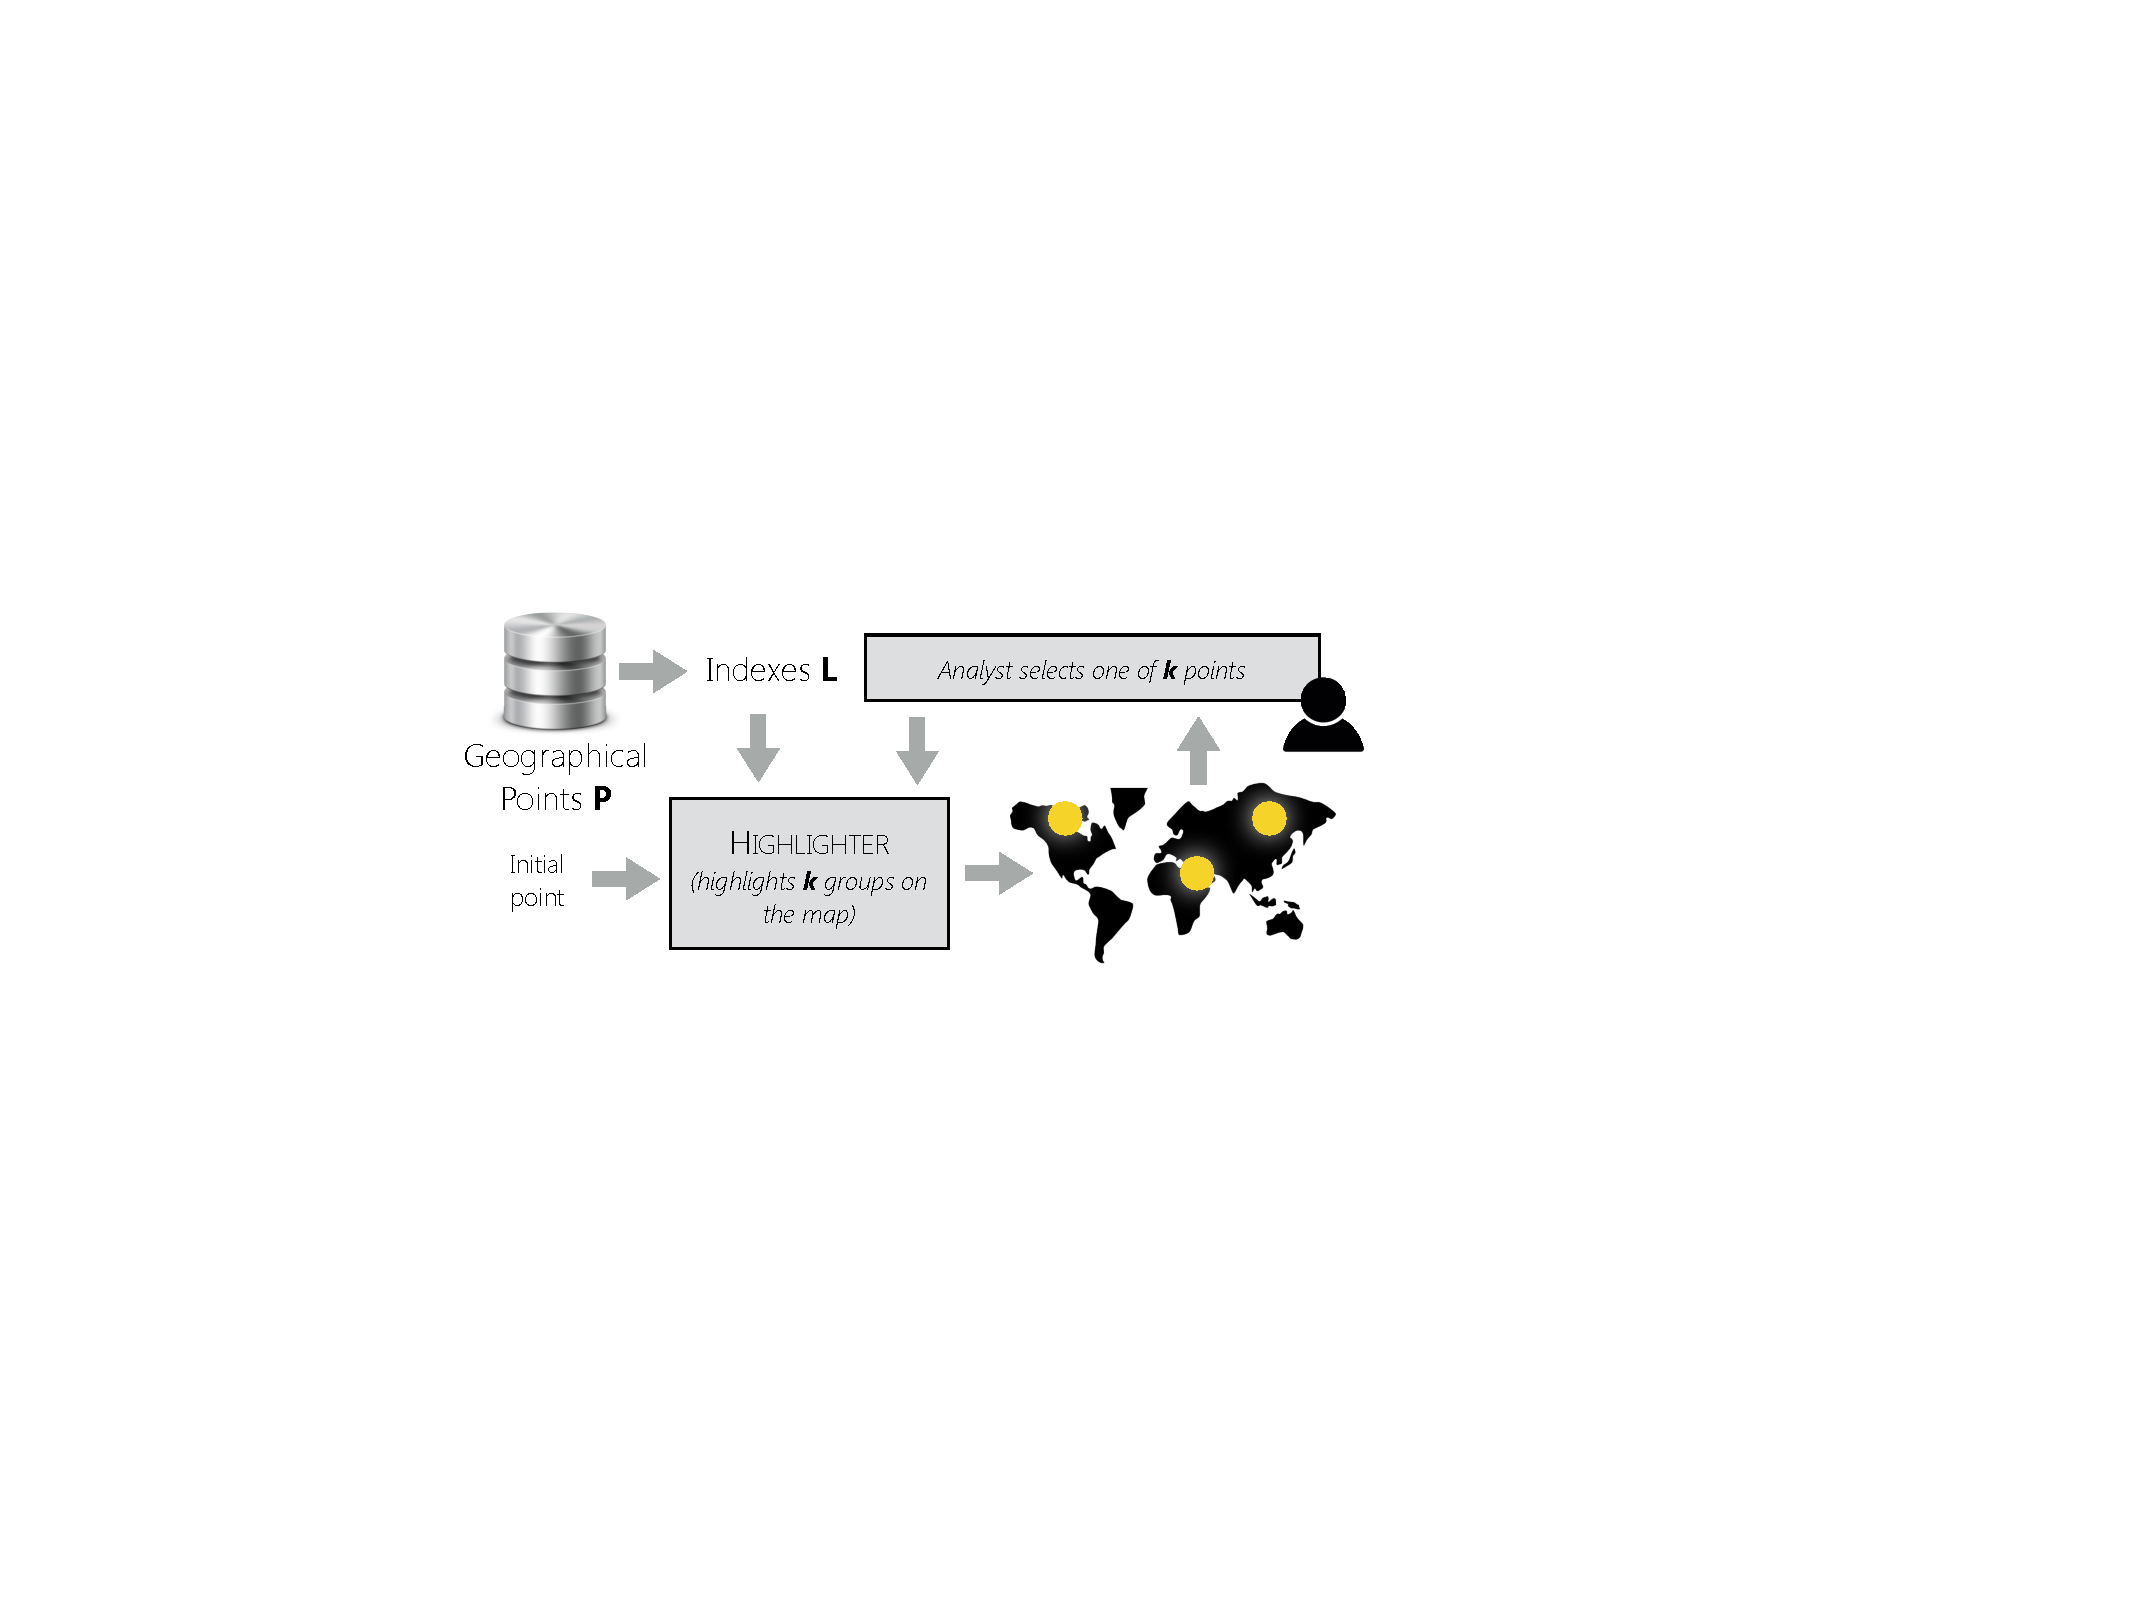
\includegraphics[width=\columnwidth]{figs/framework}

 \caption{\framework\ Framework}
 \label{fig:frame}
 \vspace{-10pt}
 \end{figure}

Figure \ref{fig:frame} illustrates the general structure of \sys. We observe that from a dataset with spatialtemporal information points, an analyst can select one of $k$ points to search for similar other points in order to proceed with specific decision like: (i) considering a Taxi analysis for pick-up a new passenger after a drop-off, \textit{which are the best points in the neighborhood to pick-up  new client?}; or (ii) considering a bicycle ride analysis, \textit{which are the best points a user can leave the bicycle considering that this user will pick-up the bike in a specific location and plan to pedal for 1 hour?} 


%\vspace{-5pt}
%\section{Running Example}
%
%...
%...
%...

\vspace{-5pt}
\section{Demonstration}

This demonstration allows to observe thoroughly the inner working of \sys, and to illustrate the use of the environment from the highlighting and guidance results in order the help the data analyst. The demonstration platform and its architecture were implemented as following: (i) the \sys engine is implemented in Python \footnote{\it https://www.python.org/}, and (ii) the graphical user interface is based on Node.js, using different libraries like \textit{D3.js\footnote{\it https://d3js.org/}, Google Maps API\footnote{\it https://developers.google.com/maps/} and Ajax\footnote{\it http://api.jquery.com/jquery.ajax/}}.  The client-side part allows the client to choose the values for a clearly-defined set of initial parameters to visualize the information about the execution of \sys with the chosen values. 


\noindent {\bf Demo.} We consider for this demonstration two realistic scenario for New York taxi\footnote{\it https://data.cityofnewyork.us/view/gn7m-em8n} and bicycle\footnote{\it https://s3.amazonaws.com/tripdata/index.html} datasets. These datasets has been frequently exploited for urban analysis
% \cite{ferreira2013visual,DBLP:journals/debu/FreireCVZ16}.
(e.g. in \cite{DBLP:journals/debu/FreireCVZ16}).
The  New York taxi dataset contains 173,179,759 records of taxi trips and 18 attributes such as pickup and dropoff date/time, passenger count and trip distance. The New York bicycle dataset contains information from 2013 to 2016, and 15 attributes such as start station id and end station id, their respective geographical informations, trip duration and distance.
% The dataset size is 27.9 GB with informations of trips from 2014.
These scenarios illustrate how an analyst can achieve an exploratory analysis goal. We preprocessed the original datasets and considered a subset of 20K unique points for the sake of clarity of results.

\noindent {\bf Scenario 1.} The scenario consists of a data scientist, we name Lucas, whose task is to optimize New York taxi trips. Focusing on cab-idle locations, he wants to discover which neighborhoods work the best for which drivers to increase the overall availability. Also, he goals to discover how drivers should choose their next cab-idle station to be more available. Lucas employs \framework\ and follows a case-by-case inspection as his analysis methodology by analyzing and learning from historical data. Considering this,  we present how \sys can support Lucas by retrieving quality information to his analysis. Figures \ref{fig:dashboard} and \ref{fig:dashboard2} present the \sys dashboard for this scenario, where the analyst can choose a initial point from a set of points. Then, the framework the presents $k$ other potential points that may be consider in Lucas analysis from the set of parameters ($\sigma, k$ and a $timeLimit$) defined. The same process can be made again in a \textit{second pass}. 


 \begin{figure}[!ht]
   \centering
   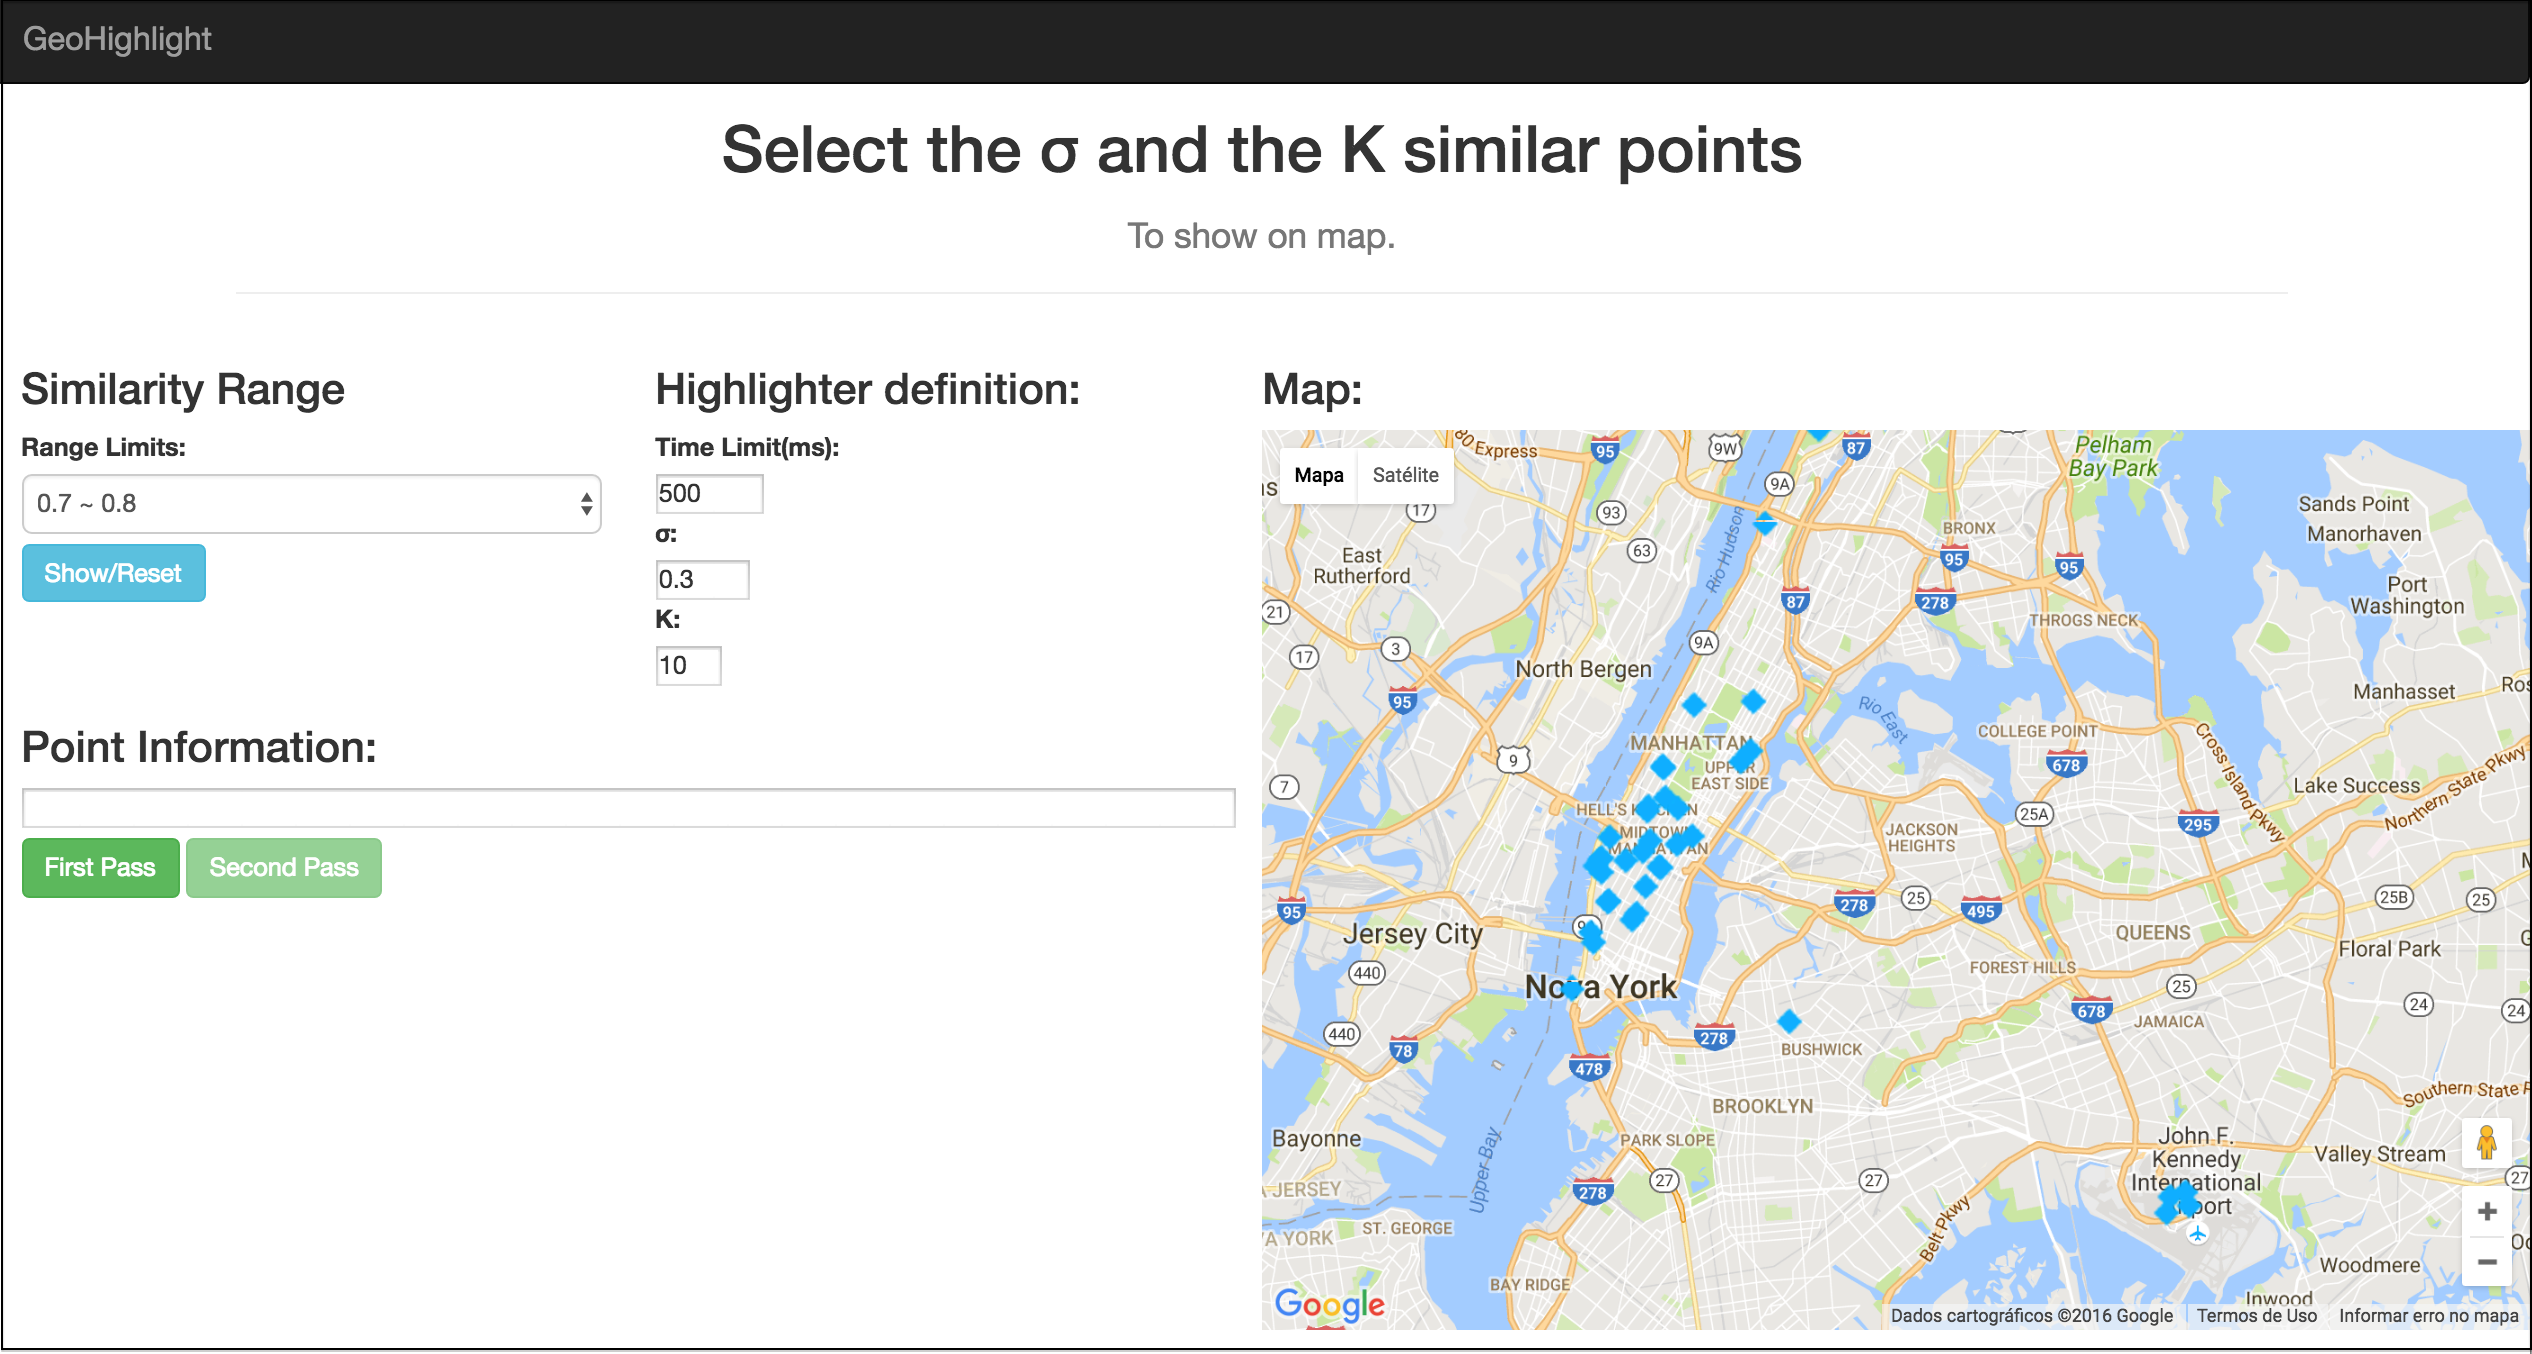
\includegraphics[width=\columnwidth]{figs/dashboard1}
 \caption{\framework\ Dashboard [New York Taxi Scenario] - View of a set of taxi pick-up and drop-off points.}
 \label{fig:dashboard}
 \vspace{-10pt}
 \end{figure}

 \vspace{-5pt}
  \begin{figure}[!ht]
   \centering
   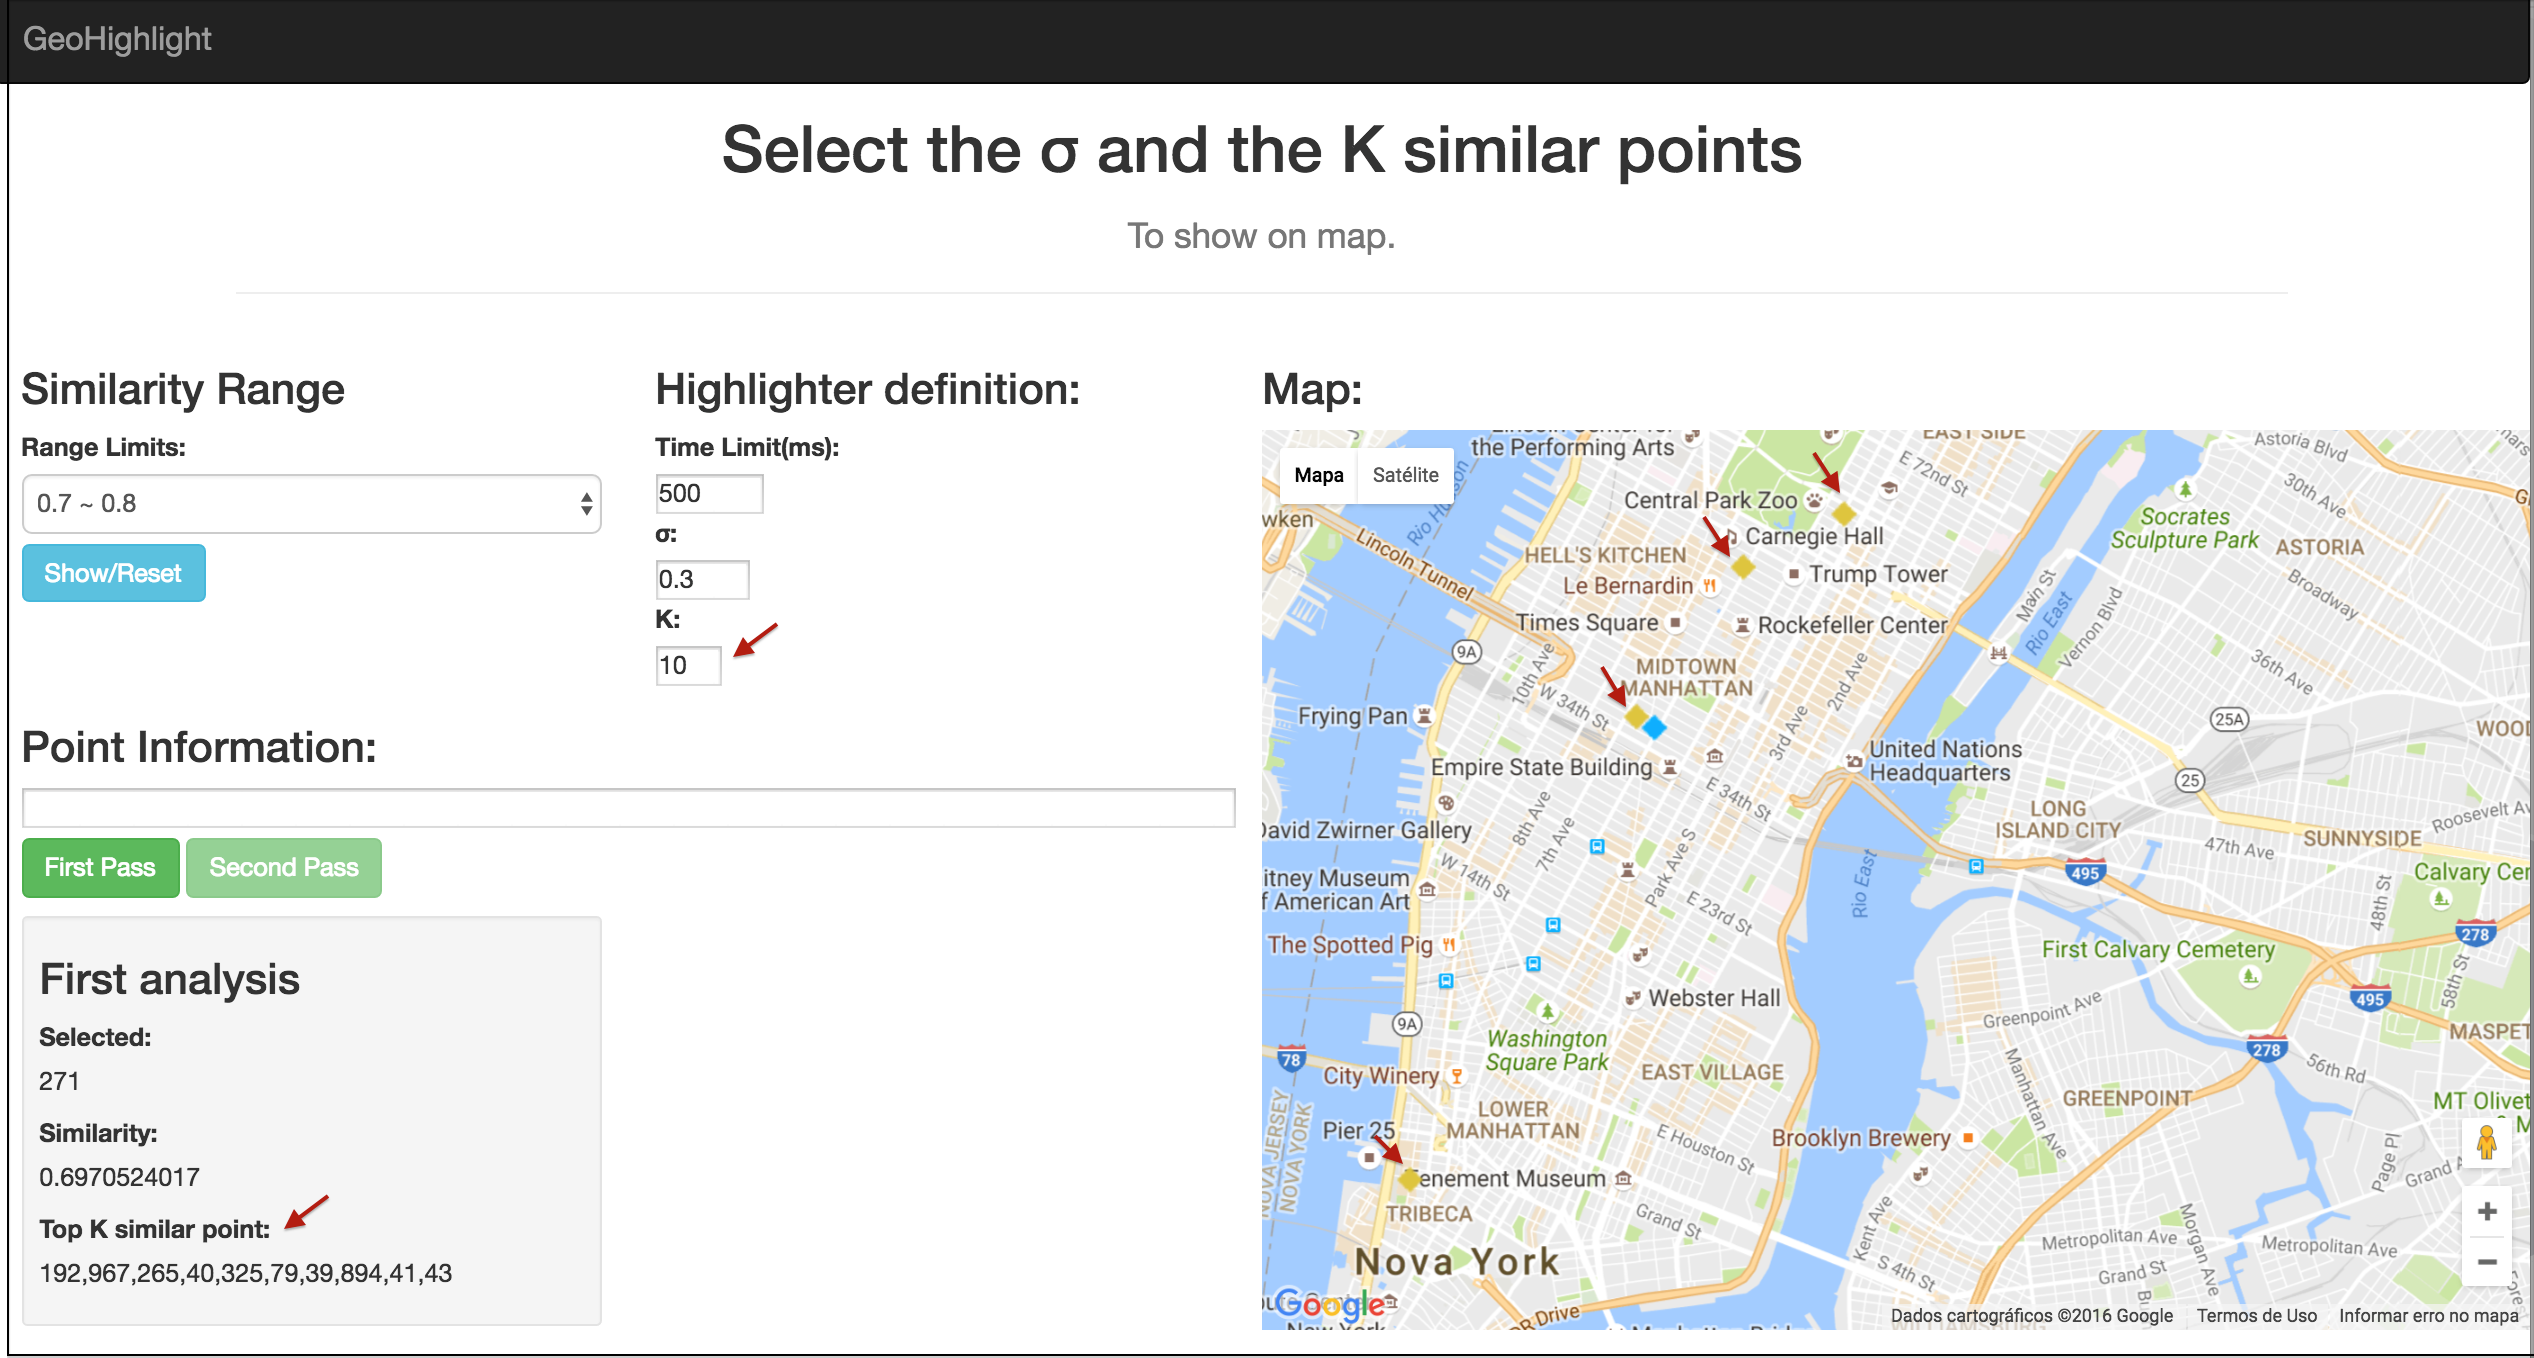
\includegraphics[width=\columnwidth]{figs/dashboard2}
 \caption{\framework\ Dashboard [New York Taxi Scenario] - Choosing a specific point from $\sigma, k$ and a $timeLimit$.}
 \label{fig:dashboard2}
 \vspace{-10pt}
 \end{figure}
 
 
\noindent {\bf Scenario 2.} Another data scientist, we name Shadi, whose task is to optimize New York bicycles station location in New York by analysing the rides from January until September 2016. How to identify problems considering the day and time for drop-off  bike rides in full stations. She must to identify the problematic bike stations to pick-up and drop-off .
 
 \section{Conclusion}
 
 In this demo we have presented \sys, a generic and interactive
framework for visualization of spatiotemporal data. Some future extensions include the integration
of generic query approach based on \cite{VartakRMPP15}, and we also want to consider an analyst profile vector which is built during interactive steps and will be exploited to return more analyst-tailored results.


\bibliographystyle{abbrv}
\bibliography{main}




% that's all folks
\end{document}


